\begin{center}
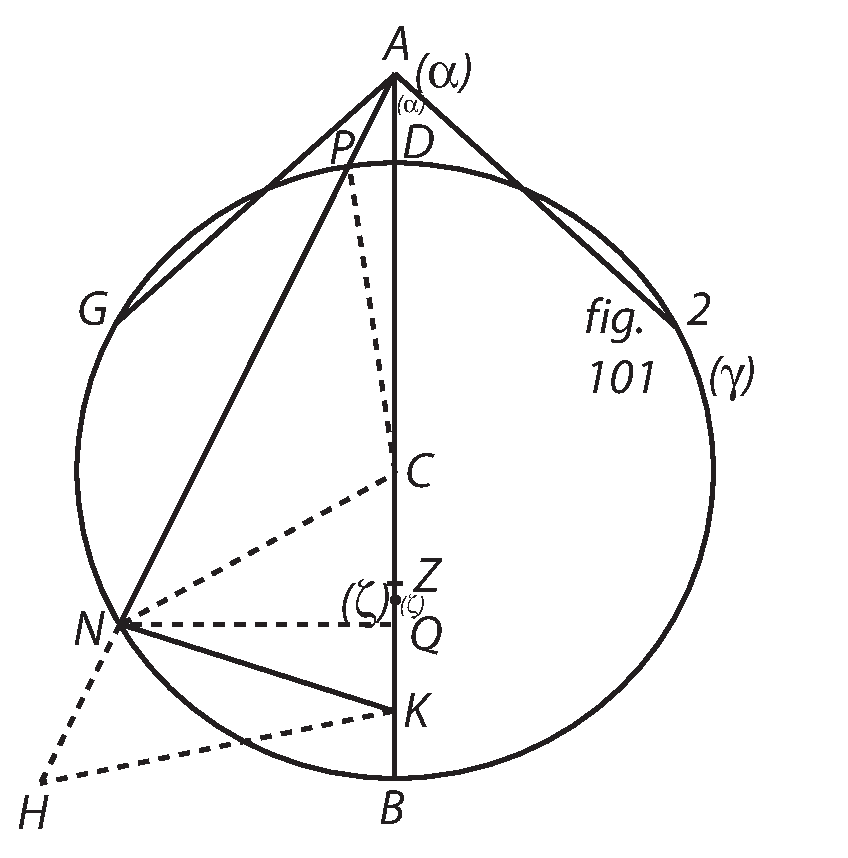
\includegraphics[width=0.4\textwidth]{images/T8_Barrow-2}
\\ \textit{[Fig. 2]} \footnote{\textit{Unterhalb von fig. 101}: \raisebox{-2ex}{ \renewcommand{\arraystretch}{2.0} \protect\begin{tabular}{c}$\displaystyle\frac{CZ}{CB}$ aequ. $\displaystyle\frac{AC}{AB}$\\$CK$ majus $CZ$\end{tabular}}}
\newpage
\includegraphics[width=0.3\textwidth]{images/T8_Barrow-1}
\\ \textit{[Fig. 1]} \footnote{\textit{Oberhalb von fig. 97:} \textit{AN} aequ. \textit{AC}}
\end{center}